\section {Implementation and Technical Notes}

Python 3.6 was used to code, with modularity of components being the main focus. Questions may be run as:

\begin{lstlisting}
    python3 main --question q
\end{lstlisting}

with questions numbered from 1 to 7. The tarball also contains a dockerfile, which maybe used to replicate results.

\subsection{Modularity of Code}

Following modules are used:
\begin{itemize}
\item  \textit{Activations}
\item \textit{Confusion Matrix}
\item \textit{MNIST Downloader}
\end{itemize}

\subsection{Directories}
The following directories are meant for specific purposes:
\begin{itemize}
\item  \textit{data}: stores MNIST zip files
\item \textit{logs}: stores plots and outputs.
\item \textit{models}: stores .npz files, which are weights of the trained model (if saved).
\end{itemize}

\section {Question 1 and 2}

Implemented a feedforward network (Multilayer Perceptron) in numpy.

Used the MNIST Dataset with the following folds:
\begin{itemize}
\item Training Dataset, original 60k images
\item k-Fold Dataset of 2k each, total 5 folds.
\end{itemize}

We shuffle both the train and fold datasets, and the first four folds are used as validation sets. 

Network initialisation is done with random normal distributions of small variations ($\sigma = 0.08$ or lesser).

We obtain the following training loss and accuracy curves.

Notice that no regularisation was used, accounting for the overfitting nature of the MLP.

\begin{figure}[ht]
\centering
%%\includegraphics[angle=0,width=0.8\textwidth]{Figure_1.png}
\caption{Loss curves for \textbf{MLP with sigmoid activations}}
\end{figure}

\begin{figure}[ht]
\centering
%%\includegraphics[angle=0,width=0.8\textwidth]{Figure_1.png}
\caption{Loss curves for {MLP with sigmoid activations}}
\end{figure}

For part 2, we run metric evaluations on all 5 folds of the test-validation set.

We report the following: (for each fold)

\begin{itemize}
\item  Confusion Matrix
\item Accuracy
\item F1 Score (per class)
\item Precision (per class)
\item Recall (per class)
\end{itemize}

For brevity, metrics are not shown for all folds. They may be recovered by running

\begin{lstlisting}
    python3 main --question 1
\end{lstlisting}

\begin{lstlisting}[numbers=none]
cm [[ 773.    0.    7.    1.    0.    4.    9.    1.    7.    1.]
 [   0.  845.    1.   23.    0.    0.    3.    0.   48.    4.]
 [   8.    0.  728.   27.    8.    1.    9.    1.   37.    6.]
 [   0.    0.    2.  728.    1.   22.    0.    2.   27.   10.]
 [   3.    0.    5.    6.  667.    3.   12.    0.   30.   48.]
 [  11.    0.    5.   30.    2.  630.    7.    1.   30.   12.]
 [   9.    1.    2.    0.    2.   10.  724.    0.   10.    2.]
 [   5.    0.   96.   10.    6.    2.    0.  629.    8.   62.]
 [   2.    0.    3.   12.    5.    8.    5.    3.  714.   13.]
 [   6.    2.    5.   15.   20.   15.    0.    3.   29.  716.]] 
 accuracy 0.94425
 precision [ 0.94614443  0.99646226  0.85245902  0.85446009  0.93811533  0.90647482
  0.94148244  0.9828125   0.75957447  0.81922197]
 recall [ 0.9626401   0.91450216  0.88242424  0.91919192  0.86175711  0.86538462
  0.95263158  0.76894866  0.93333333  0.88286067]
 F1_score [ 0.95432099  0.9537246   0.86718285  0.88564477  0.8983165   0.88545327
  0.9470242   0.86282579  0.83753666  0.84985163]
\end{lstlisting}


\subsection {Code Blocks (Forward and Backward Pass)}
\begin{lstlisting}
 def _forward_prop(self, x):
        '''
        RUn forward prop.
        '''
        a = np.array(x).reshape((len(x),1))
        for count, b, w in zip(range(self.num_layers-1),self.biases, self.weights):
            if count==self.num_layers-2:
                a = activations.softmax(np.dot(w, a)+b)
            else:
                a = self.activation(np.dot(w, a)+b)
        return a

    def _back_prop(self, x, y):
        """
        Compute gradients of Cost
        
        Returns:
        * (nabla_b, nabla_w) representing the
        gradient for the cost function C_x.  
        
        nabla_b and nabla_w are similar
        to self.biases and self.weights.
        """
        nabla_b = [np.zeros(b.shape) for b in self.biases]
        nabla_w = [np.zeros(w.shape) for w in self.weights]

        # backward pass
        delta = self.cost_derivative(a_ss[-1], y) * activations.softmax_prime(zs[-1])

        nabla_b[-1] = delta
        nabla_w[-1] = np.dot(delta, a_ss[-2].transpose())
        
        for l in range(2, self.num_layers):
            delta = np.dot(self.weights[-l+1].transpose(), delta) * self.activation_prime(zs[-l])
            #print(delta)
            nabla_b[-l] = delta
            nabla_w[-l] = np.dot(delta, a_ss[-l-1].transpose())

        return (nabla_b, nabla_w)
\end{lstlisting}

We run the list of properties for all possible GPU's present in the given machine.

\bigskip
\newpage

\subsection{Running a Test Image}

This is originally a part of question 5, but has been integrated into questions(1-2) , question(3), and question(4).

The full outputs may be recovered by running

\begin{lstlisting}
    python3 main --question 1
\end{lstlisting}

For brevity, a sample output is shown here:

\begin{figure}[ht]
\centering
%%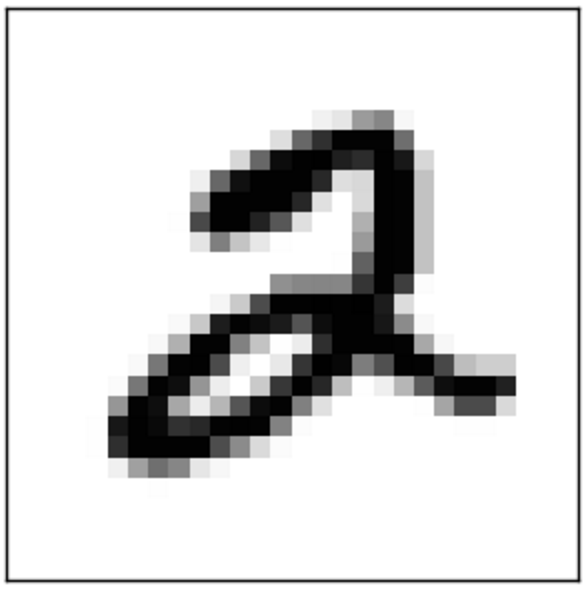
\includegraphics[angle=0,width=0.8\textwidth]{assign-1/report/mnistimg.jpg}
\caption{Sample MNIST digit. Y true =2 , Y pred =2 , probability (softmax) =0.91}
\end{figure}

\section {Question 3 }
\noindent We use relu activation layers instead of sigmoid for training the MLP. \\

\textbf{Question 3} involves using smaller variances to ensure no exploding gradients while using relu.  We however observe faster and better convergence with relu. This could be attributed to the nearly linear nature of the activation and the fact that it does not die for large values.\\

The relevant metrics:

\begin{lstlisting}[numbers=none]
test loss 0.49272746608690554
cm [[ 170.    0.    3.    1.    0.    0.    3.    0.    0.    0.]
 [   0.  197.    0.    5.    0.    0.    1.    0.    7.    1.]
 [   0.    0.  184.    7.    1.    0.    3.    0.    9.    3.]
 [   0.    0.    2.  199.    0.    8.    0.    0.    4.    5.]
 [   0.    0.    1.    2.  180.    1.    3.    0.   10.   11.]
 [   0.    0.    0.    7.    0.  145.    2.    0.    9.    1.]
 [   3.    1.    1.    0.    2.    2.  185.    0.    3.    1.]
 [   0.    0.   18.    4.    1.    4.    0.  161.    4.   18.]
 [   0.    0.    2.    3.    5.    1.    0.    1.  196.    1.]
 [   0.    0.    1.    6.    9.    4.    2.    0.    6.  170.]]
 accuracy 0.9635
 precision [ 0.98265896  0.99494949  0.86792453  0.85042735  0.90909091  0.87878788
  0.92964824  0.99382716  0.89032258  0.8056872 ]
 recall [ 0.96045198  0.93364929  0.88888889  0.91284404  0.86538462  0.88414634
  0.93434343  0.76666667  0.93779904  0.85858586]
 F1_score [ 0.97142857  0.96332518  0.87828162  0.88053097  0.88669951  0.88145897
  0.93198992  0.8655914   0.85776805  0.83129584]
\end{lstlisting}

\section {Question 4}

Here, we empirically investigate the dependence of run-time on the number of operations per thread.

\subsection{Code Changes} 
\begin{lstlisting}
	__global__ void VecAdd(float* A, float* B, float* C, int N){
      // Host code
      int j;
    int i = blockDim.x * blockIdx.x + threadIdx.x;
    if (i < N_op){
        for (j=0;j<op_loop;j++)
            C[i*op_loop+j] = A[i*op_loop+j] + B[i*op_loop+j];
    }
    }
   // Array of op's to try//
   for (op_loop_ii=0;op_loop_ii<10;op_loop_ii++){
        op_loop_array[op_loop_ii]=pow(2,op_loop_ii);
    }
// Run kernel over these ops and average each run //
cudaEventRecord(start, 0);
VecAdd<<<blocksPerGrid, threadsPerBlock>>>(d_A,d_B, d_C, N);
cudaEventRecord(stop, 0);
cudaEventSynchronize(stop);
cudaEventElapsedTime(&time_spent, start, stop);
time_spent=time_spent/(avg_loop-1)*10;
\end{lstlisting} \\

\subsection{

\subsection{Reasoning}

The optimal operations per block is dependent on the level of SIMD parallelism a single thread may be able to achieve. With an optimal of \textbf{4}, it is possible that the device has over \textbf{8 ALU's} per thread-context. \\

\section {Question 6 and 7}

Here, we use the \textbf{Histogram of Oriented Gradients} as the feature extractor before using a classifier. In \textbf{Question 6}, we try a MLP based classifier having
